\begin{figure}[!t]
\centering
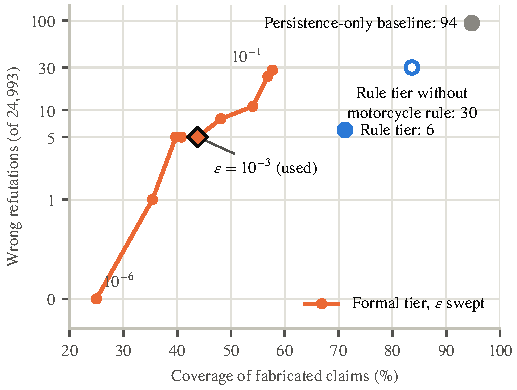
\includegraphics[width=\columnwidth]{fig_errcov.pdf}
\caption{Pre-registered generalization test (G1--G4 pooled; 24,993 genuine and 10,551 empty claims): wrong refutations (symmetric-log scale) against coverage of fabricated claims. The formal tier is swept over $\varepsilon \in \{10^{-1}, 3\cdot10^{-2}, 10^{-2}, 3\cdot10^{-3}, 10^{-3}, 3\cdot10^{-4}, 10^{-4}, 10^{-5}, 10^{-6}\}$; the diamond marks the operating point $\varepsilon = 10^{-3}$. The rule tier gives the same point for persistence counts $k_s = 2$--6. Simulated data.}
\label{fig:errcov}
\end{figure}
